\documentclass[dvipdfmx,a4j, titlepage]{jsarticle}
\usepackage{listings,jvlisting,array,tcolorbox,ascmac,siunitx,amsmath,amssymb,bm,here,float,comment,url}

% 以下の内容を記載
% 1. 表紙(名前と学籍番号含む)
% 2. 仕様書(何を作ったか.何故作ったか.どのように作ったか.)
% 3. 回路の説明(全体図は必ず入れる.部分的な図は説明に必要なものは入れる.)
% 4. 考察,まとめ
% 5. 感想,学び

% TODO: 
% - 学籍番号の挿入
% - 回路図pdfの結合

\title{電気電子工学実験3 テーマS(a)\\ 簡単な4bit CPUの製作}
\author{三木 健太郎}
\date{2023年11月20日}
 
\begin{document}

\maketitle

\section{概要}
\subsection{製作物の概要}
本テーマ後半の自由設計では、簡単な4bit CPUの製作を行った。
このCPUはデータ転送命令や加算命令、データの入出力命令などを実行することができる。
これらの命令を組み合わせることで、LEDを予め決めた通りのパターンで光らせるプログラムや、
タイマー機能を持つプログラムなどを実行することができる。

\subsection{書籍「CPUの創りかた」について}
74シリーズの汎用論理ICを用い、データ転送・加算・データ入出力といった命令を実行できる4bit CPUを製作する方法を解説した書籍である。
LEDの点灯回路といった基本的な事項から、CPUの基本構成、実装方法といった応用的な事項まで、幅広い内容が平易に解説されている。
2003年に毎日コミュニケーションズ(現 マイナビ出版)から出版され、現在30刷以上重版されている。

\subsection{製作の動機}
計算機工学1や2で、フリップフロップなどのディジタル回路の基本的な構成要素やCPUの構造について学習した。
しかし、授業で知識を学んだだけでは、CPUの内部構造について、深い理解を得ることはできなかった。
そこで、本実験において簡単なCPUを実装することにより、CPUの内部構造を実感をもって理解したいと考えた。
簡単なCPUを実装するという内容の書籍は複数存在するが、回路自体の規模が大きく、授業時間内で実装を完遂するのが難しいものが多かった。
「CPUの創りかた」で解説されている「TD4」は、機能を絞っている分、回路の規模が小さく、授業時間内で実装を完遂することが可能であると考えた。

\subsection{制作方法}
基本的には、書籍「CPUの創りかた」に従って製作を行った。
具体的には、レジスタ、ALU、プログラムカウンタ、命令デコーダ、ROMの順に実装を行った。
書籍では74シリーズのICを用いながら実際に回路を組み立てるため、
解説内容がFPGAでの実装にそぐわない部分が一部あった。
そのような部分については、FPGAでの実装に適した内容に書き換えた。(詳細は後述する。)

\section{回路の説明}
\subsection{TD4の仕様}
TD4の命令長は8bitとなっており、オペコードが4bit、オペランドが4bitとなっている。
\footnote { 表現できるアドレスも4bitの範囲となるため、実行できるプログラムは最大で16ステップのものまでとなる。 }
演算用のレジスタはAレジスタとBレジスタの2つあり、いずれも4bitの値を記憶することができる。\\
TD4において実行できる命令の一覧を、 以下の表\ref{instruction_list}に示す。

\begin{table}[hbtp]
    \caption{TD4で実行可能な命令の一覧}
    \label{instruction_list}
    \centering
    \begin{tabular}{ccc}
        \hline
        命令                                  & オペコード & 概要                                                                       \\
        \hline \hline
        \verb|ADD A, Im|                & 0000       & Aレジスタに即値\verb|Im|を加算する                            \\
        \verb|ADD B, Im|                & 0101       & Bレジスタに即値\verb|Im|を加算する                            \\
        \verb|MOV A, Im|                & 0011       & Aレジスタに即値\verb|Im|を代入する                            \\
        \verb|MOV B, Im|                & 0111       & Bレジスタに即値\verb|Im|を代入する                            \\
        \verb|MOV A, B|                & 0001       & Bレジスタの値をAレジスタに代入する                                         \\
        \verb|MOV B, A|               & 0100       & Aレジスタの値をBレジスタに代入する                                         \\
        \verb|JMP Im|               & 1111       & 即値\verb|Im|で指定されたアドレスにジャンプする              \\
        \verb|JNC Im|               & 1110       & キャリーフラグが0のとき即値\verb|Im|のアドレスにジャンプする \\
        \verb|IN A|               & 0010       & 入力端子からデータを入力し、Aレジスタに代入する                            \\
        \verb|IN B|               & 0110       & 入力端子からデータを入力し、Bレジスタに代入する                            \\
        \verb|OUT B| \footnotemark & 1001       & Bレジスタの値を出力端子に出力する                                          \\
        \verb|OUT Im|               & 1011       & 即値\verb|Im|を出力端子に出力する                            \\
        \hline
    \end{tabular}
\end{table}
\footnotetext{なお、\verb|OUT A|命令は存在しない。}

\subsection{回路の全体像}
今回製作した回路の全体像を、以下の図\ref{circuit_diagram}に示す。なお、高解像度の回路図を本レポートの末尾に付した。

\begin{figure}[H]
    \begin{center}
        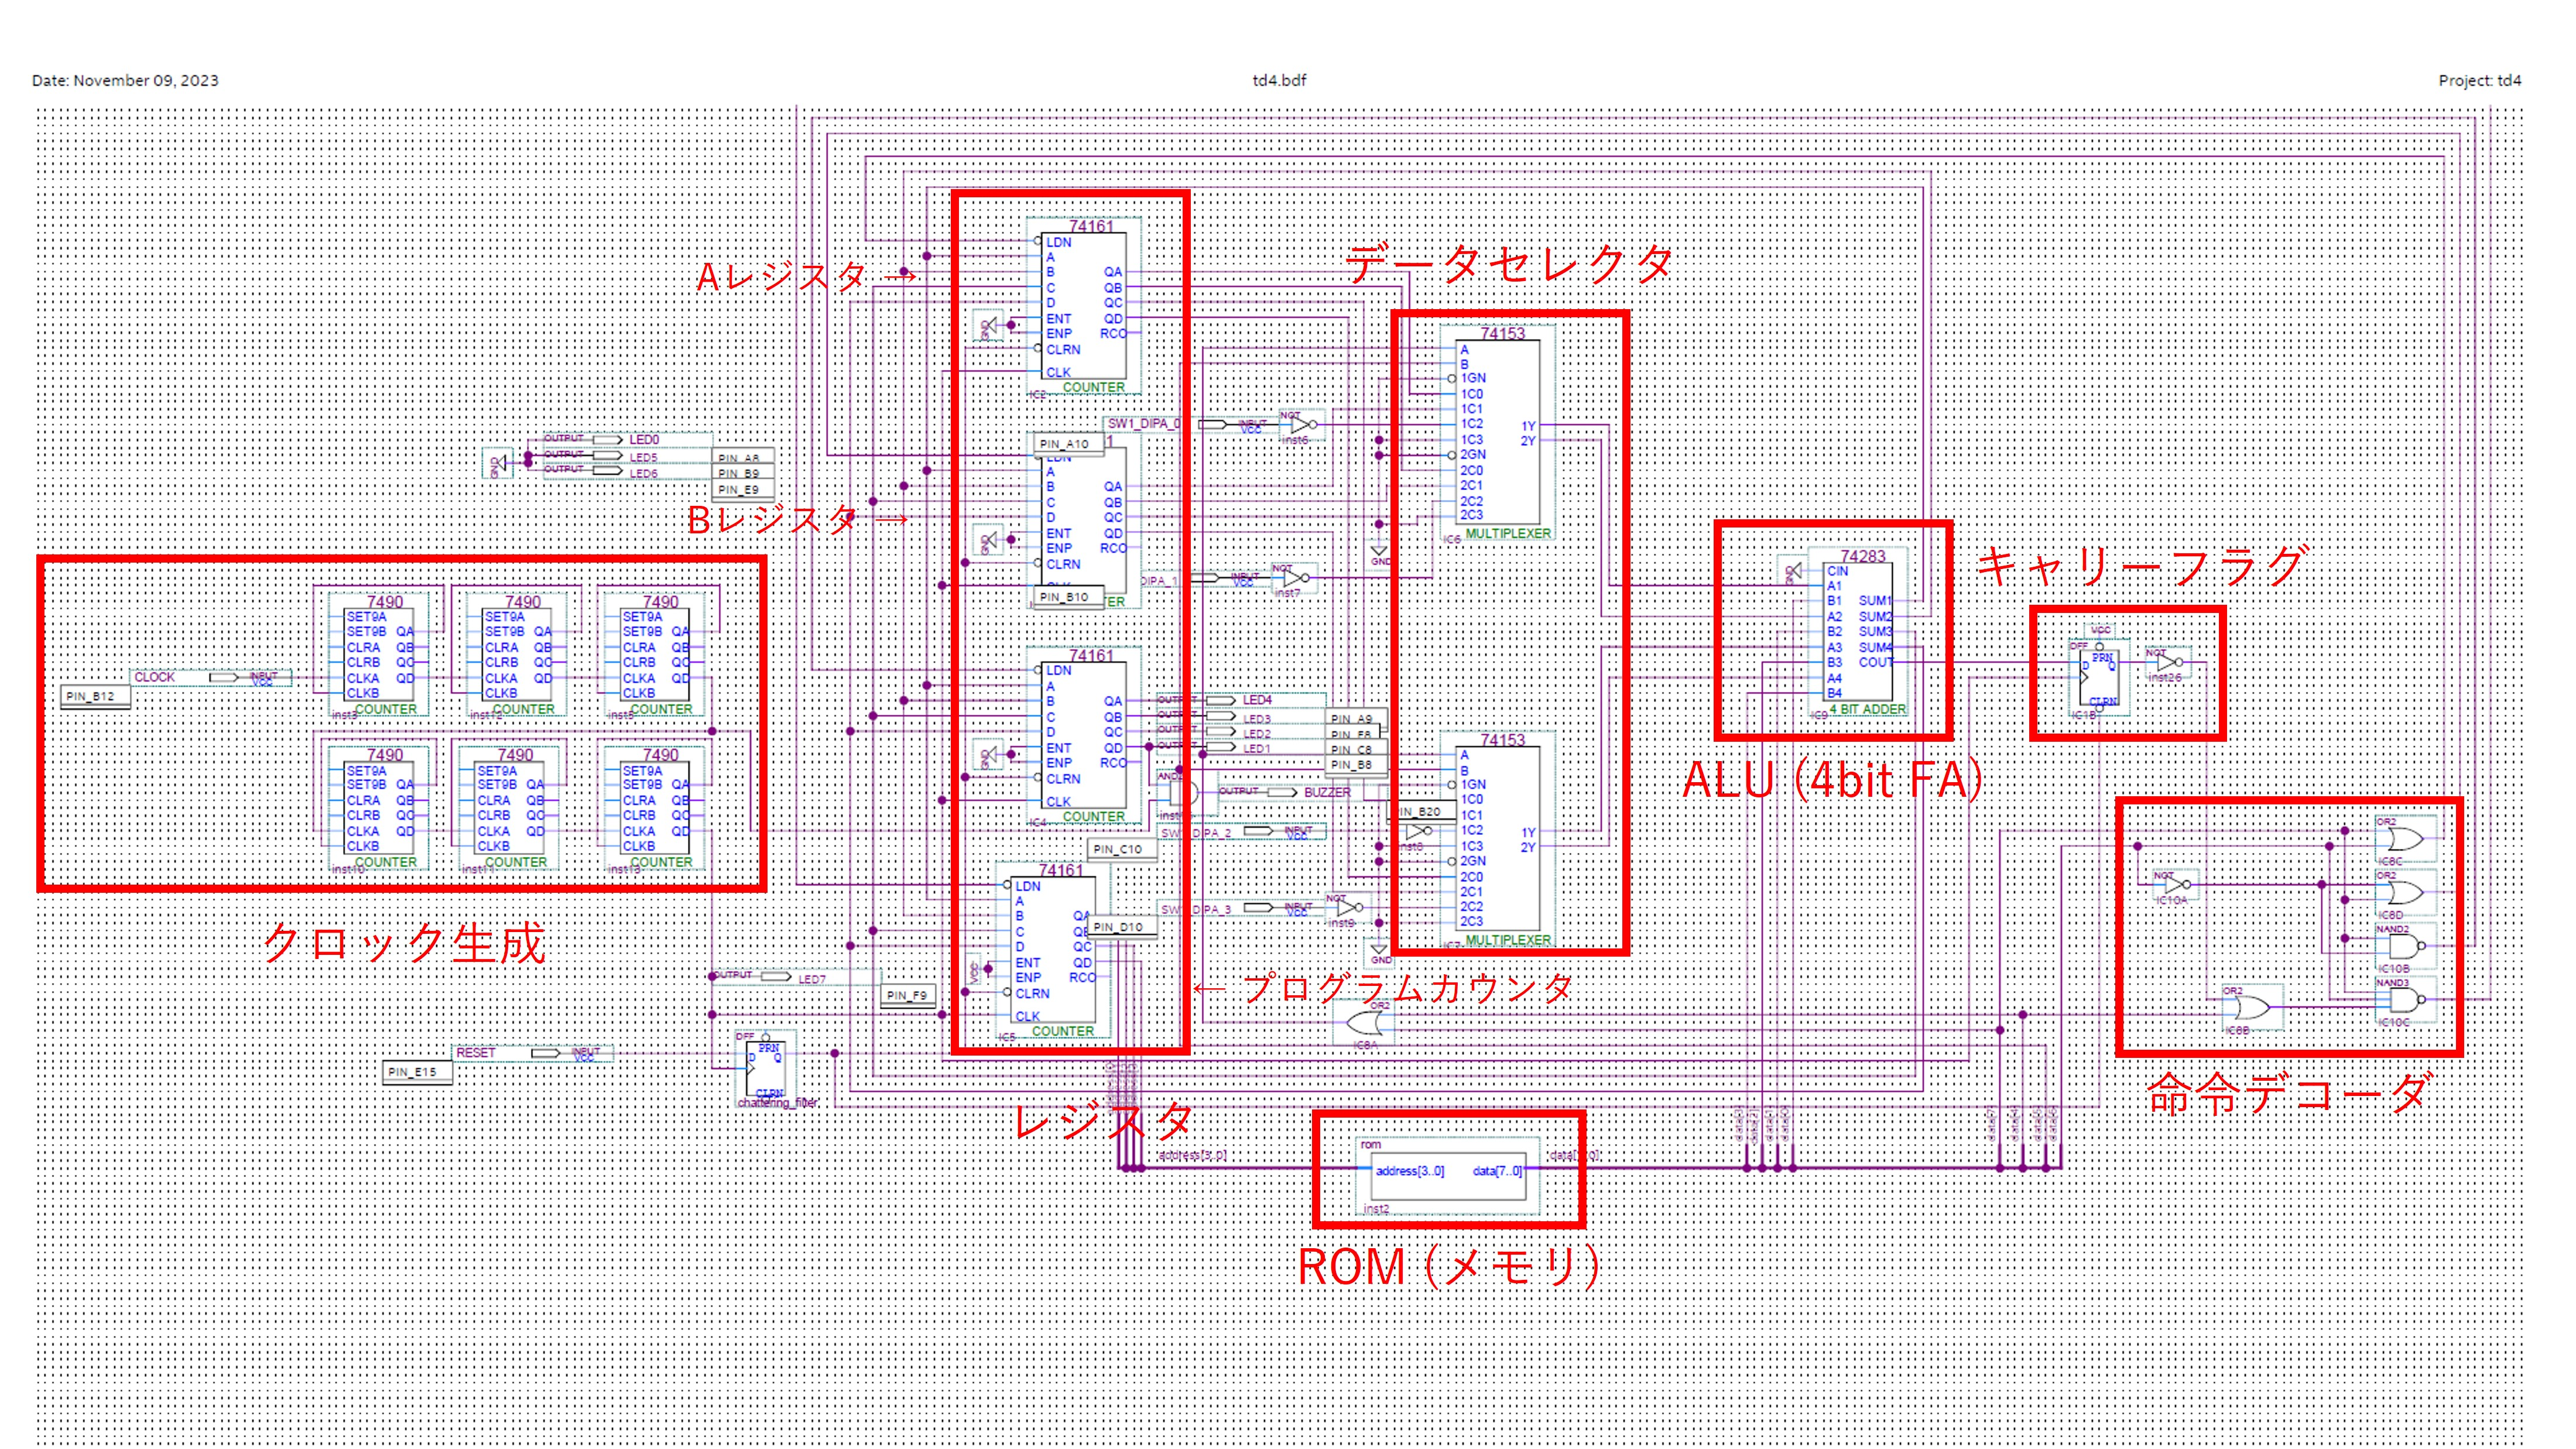
\includegraphics[width=165mm]{img/circuit_diagram.jpg}
    \end{center}
    \caption{製作した回路の全体像}
    \label{circuit_diagram}
\end{figure}

図\ref{circuit_diagram}の"クロック生成"と書かれた部分では、7490を用いて評価ボード(MU500-RXSET01)の生成するクロックを、人間にも確認しやすい程度の周波数(数Hz程度)に落としている。\\

"レジスタ"は、プログラムの実行に必要な値やアドレスを格納している。上の2つのレジスタは演算用のレジスタであり、ROMから読みだした値やアドレスを格納したり、ALUでの演算結果を格納したりするのに用いられる。また、その下のレジスタは出力端子に直結しており、出力端子に出力する値を保持するために用いられている。一番下のレジスタはプログラムカウンタであり、現在CPUが実行している命令のアドレスを記憶している。\\

その右の"データセレクタ"は、命令デコーダの出力を元に、指定されたレジスタから値を読み出し、ALUへと送る役割を担っている。\\

"ALU"は、Arithmetic Logic Unit (算術論理演算装置)の略であり、算術演算や論理演算を行う回路である。今回製作したCPUでは、算術命令は\verb|ADD|命令(加算命令)しか存在しないため、ALUとして単に74283 (4bit全加算器)を用いている。\\

"命令デコーダ"は、ROMから読みだした命令の上位4bitのオペコードを見て、データセレクタがデータを読み出すべきレジスタを指定するとともに、各レジスタに対して値をロードするか保持するかを決定している。\\

"キャリーフラグ"は、D-FFを用いて\verb|ADD|命令において繰り上がりが発生した場合に、繰り上がりが発生したことを示すフラグ(キャリーフラグ)を記憶している。ここで記憶されたフラグは、\verb|JNC|命令において、オペランドとして受け取ったアドレスにジャンプするかどうかの判定に用いられる。\\

"ROM"は、Read Only Memoryの略であり、CPUで実行するプログラムを記憶している。この回路のROMは16個のアドレス空間を持ち、アドレス1つ1つに対して命令が記録されている。例えば、ROMの\verb|0010|番地に\verb|01010010| (=\verb|ADD B, 2|)という命令が記録されていた場合、プログラムカウンタが\verb|0010|を指したときに、CPUはBレジスタに2を加算する命令を実行する。ROMの実装の詳細については、\ref{implemtnt_rom}節で述べる。\\

\subsection{CPUの動作の流れ}
CPUはリセットがかかると、ROMの\verb|0000|番地の命令から実行を開始していく。ROMに記録されている機械語命令のうち、上位4bitはオペコード(命令の種類)を表しており、下位4bitはオペランド(演算に用いる値やアドレス)を表している。オペコードは命令デコーダに読み込まれ、オペランドはALUに送られる。次に、読み込んだオペコ―ドやオペランドを元に命令を実行する。例えば、ALUで加算を行ったり、レジスタに値をロードしたりする。演算結果はレジスタに格納され、次以降の命令に利用する。最後にプログラムカウンタの値を1増加させ、次に\verb|0001|番地の命令を同様に実行する。こうした動作をクロックに合わせて繰り返し行うことで、CPUは動作する。

\subsection{ROMの実装方法}\label{implemtnt_rom}

\end{document}
